% Build twice here: pdflatex -interaction=nonstopmode -halt-on-error resume12An26w.tex
\documentclass[a4paper,10pt,pdflatex,ja=standard,jafont=ipaex-type1,
  magstyle=real,scale=1]{bxjsarticle}
\usepackage{lmodern}
\usepackage{amsmath,amssymb,mathtools}
\usepackage{geometry}
\geometry{reset,left=22mm,right=22mm,top=20mm,bottom=17mm,
  headheight=13pt,headsep=6mm,footskip=10mm}
\usepackage{xcolor}
\usepackage{enumitem}
\usepackage{array,booktabs,tabularx}
\usepackage{fancyhdr}
\usepackage{lastpage}
\usepackage{tikz}
\usetikzlibrary{arrows.meta,calc,decorations.pathreplacing}

\definecolor{ink}{HTML}{193A5C}
\definecolor{accent}{HTML}{237D82}
\definecolor{soft}{HTML}{EAF3F3}
\definecolor{muted}{HTML}{52616B}
\newcommand{\coursename}{解析学 II}
\newcommand{\handoutnumber}{12}
\pagestyle{fancy}
\fancyhf{}
\fancyhead[L]{\small\color{ink}\coursename{}・授業要約と演習}
\fancyhead[R]{\small\color{ink}第\handoutnumber 回}
\fancyfoot[C]{\small\color{ink}\thepage/\pageref{LastPage}}
\renewcommand{\headrulewidth}{0.3pt}
\setlength{\parindent}{0pt}
\setlength{\parskip}{2pt}
\setlength{\abovedisplayskip}{5pt}
\setlength{\belowdisplayskip}{5pt}
\setlength{\abovedisplayshortskip}{3pt}
\setlength{\belowdisplayshortskip}{4pt}
\setlist[itemize]{leftmargin=1.8em,itemsep=1pt,topsep=2pt,parsep=0pt}

\newcommand{\handouttitle}[1]{%
  \begin{center}
    {\Large\color{ink}#1}\par\vspace{3mm}
    {\color{accent}\rule{0.88\linewidth}{0.7pt}}
  \end{center}\vspace{-2mm}}
\newcommand{\handout}[2]{%
  \renewcommand{\handoutnumber}{#1}%
  \handouttitle{第#1回\quad #2}}
\newcommand{\topic}[1]{\par\vspace{5pt}%
  {\large\sffamily\mdseries\color{accent}#1}\par\vspace{2pt}}
\newcommand{\keybox}[1]{\par\vspace{3pt}\begingroup
  \setlength{\fboxsep}{4pt}%
  \colorbox{soft}{\parbox{\dimexpr\linewidth-2\fboxsep\relax}{\small #1}}%
  \endgroup\par\vspace{2pt}}
\newenvironment{problems}
  {\begin{enumerate}[leftmargin=2em,itemsep=3pt,topsep=3pt,parsep=0pt,
    font=\color{accent}]}
  {\end{enumerate}}


\newcommand{\examplelabel}[1]{{\sffamily\mdseries\color{ink}#1}}
\newcommand{\problemspace}{\par\vspace{5mm}}
\newcommand{\exercises}{%
  {\color{accent}\hrule height 0.7pt}\vspace{3pt}%
  \topic{演習問題（6題）}%
  {\small 領域と積分範囲を確認し、計算過程も書こう。図を描くと範囲を読み取りやすい。}\par}
\tikzset{
  handout diagram/.style={>={Stealth[length=3.2pt,width=3.2pt]},line join=round,
    every node/.style={font=\scriptsize,text=ink}},
  region/.style={fill=soft,draw=accent,semithick},
  slice/.style={accent,line width=1.8pt},
  guide/.style={muted,densely dashed,thin},
  axis/.style={->,ink,thin}}


% Review Q&A can also be used for actual student feedback when it is available.
\newcommand{\feedback}[2]{%
  \par\addvspace{8pt}\noindent\begin{minipage}{\linewidth}%
  {\color{ink}Q. #1}\par\vspace{2pt}%
  {\color{accent}A. }#2%
  \end{minipage}\par}

\begin{document}
\fontsize{10pt}{13.5pt}\selectfont
\setlength{\abovedisplayskip}{4pt}
\setlength{\belowdisplayskip}{4pt}
% Feedback section: add comments and responses here when available.
\fancyhead[L]{\small\color{ink}\coursename{}・フィードバック}
\handout{12}{前回のコメントへのフィードバック}
% \feedback{comment}{response}
\clearpage

% Previous small-test section: add the questions and solutions here.
\fancyhead[L]{\small\color{ink}\coursename{}・小テスト}
\fancyhead[R]{\small\color{ink}第11回}
\handouttitle{第11回\quad 小テスト}
% Questions and solutions are intentionally blank.
\clearpage

\fancyhead[L]{\small\color{ink}\coursename{}・授業要約と演習}
\fancyhead[R]{\small\color{ink}第\handoutnumber 回}
\handout{12}{曲線・曲面の向き}\label{lesson-start}
\keybox{到達目標：媒介変数の順序から法線を計算し、指定された向きにそろえられる。
曲面の法線と境界曲線の向きを、図と外積の両方で確認しよう。}

\topic{曲線の向きと線積分の符号}
曲線の表示 $\vec r(t)$（$a\le t\le b$）は、$t$ の増加方向に向きを与える。
逆向きの表示は $\widetilde{\vec r}(t)=\vec r(a+b-t)$ である。
$$
 \int_{-C}\vec F\cdot d\vec r=-\int_C\vec F\cdot d\vec r,
 \qquad \int_{-C}f\,ds=\int_Cf\,ds.
$$
平面の単純閉曲線は、囲む領域を左に見る向きが正である。
開いた線分には自然な「正」の向きはなく、始点・終点で指定する。


\par\vspace{2pt}\noindent
\begin{minipage}[b]{0.48\linewidth}\centering
\begin{tikzpicture}[handout diagram,x=0.9cm,y=0.65cm]
\path[region] (0,0) circle (1.15);
 \draw[accent,->,semithick] (15:1.15) arc[start angle=15,end angle=155,radius=1.15];
 \draw[accent,->,semithick] (195:1.15) arc[start angle=195,end angle=335,radius=1.15];
 \node at (0,0) {内部は左};
 \node[below] at (0,-1.55) {反時計回り};
\end{tikzpicture}\par
{\small\color{muted}平面領域の外側の境界の正の向き}\par
\end{minipage}\hfill
\begin{minipage}[b]{0.48\linewidth}\centering
\begin{tikzpicture}[handout diagram,x=0.9cm,y=0.65cm]
\path[region] (0,0) circle (1.15);
 \draw[ink,->,semithick] (155:1.15) arc[start angle=155,end angle=15,radius=1.15];
 \draw[ink,->,semithick] (335:1.15) arc[start angle=335,end angle=195,radius=1.15];
 \node at (0,0) {内部は右};
 \node[below] at (0,-1.55) {時計回り};
\end{tikzpicture}\par
{\small\color{muted}逆向きに進むと、仕事の符号が変わる}\par
\end{minipage}
\par\vspace{2pt}

\topic{曲面の媒介変数表示と正則性}
$D\subset\mathbb R^2$ 上の $C^1$ 級写像
$\vec r(u,v)=(x(u,v),y(u,v),z(u,v))$ で曲面 $S$ を表す。
内部で $\vec r_u\times\vec r_v\ne\vec0$ なら、2本の接ベクトルは独立である。
$$
 \vec N=\vec r_u\times\vec r_v,\qquad
 \vec n=\frac{\vec N}{|\vec N|},\qquad dS=|\vec N|\,du\,dv.
$$
表示は内部で1対1とする。球面などは必要に応じて複数の座標で覆う。


\topic{曲面の向きと法線}
連続な単位法線 $\vec n$ を選べる曲面を向き付け可能という。
連結な曲面の向きは $\vec n$ と $-\vec n$ の2通り。
パラメータの順序を交換すると、外積の向きが逆になる。
$$
 \vec r_v\times\vec r_u=-\vec r_u\times\vec r_v.
$$
グラフ $z=f(x,y)$ を $(x,y)$ の順で表すと $\vec N=(-f_x,-f_y,1)$ は上向き。
閉曲面が立体を囲む場合は、外向きか内向きかを指定する。


\par\vspace{2pt}\noindent
\begin{minipage}[b]{0.98\linewidth}\centering
\begin{tikzpicture}[handout diagram,x=0.75cm,y=0.65cm]
\path[region] (-1.5,-0.45) -- (1.3,-0.1) -- (2,0.8) -- (-0.8,0.45) -- cycle;
 \draw[->,ink,semithick] (0,0.1) -- (0,1.9) node[above] {$\vec n$};
 \draw[->,muted,dashed] (0,0.1) -- (0,-1.2) node[below] {$-\vec n$};
 \draw[->,accent] (-1.5,-0.45) -- (1.3,-0.1) node[midway,below] {$\vec r_u$};
 \draw[->,accent] (-1.5,-0.45) -- (-0.8,0.45) node[midway,left] {$\vec r_v$};
 \node[right] at (2.7,0.8) {$\vec r_u\times\vec r_v$};
 \node[right] at (2.7,-0.1) {順序を逆にすると法線も反転};
\end{tikzpicture}\par
{\small\color{muted}向きを反転しても、面積要素 $dS$ の大きさは変わらない}\par
\end{minipage}
\par\vspace{2pt}

\newpage
% Keep the remaining summary in the upper half of page 2.
\noindent\begin{minipage}[b][\dimexpr0.5\textheight-\parskip\relax][t]{\linewidth}
\topic{例：円柱と球面を外向きに表す}
半径1の円柱側面では $\vec r(\theta,z)=(\cos\theta,\sin\theta,z)$ とすれば
$$
 \vec r_\theta\times\vec r_z=(\cos\theta,\sin\theta,0)
$$
は外向きである。
球面では $\vec r(\alpha,\theta)=(\sin\alpha\cos\theta,\sin\alpha\sin\theta,\cos\alpha)$ として
$$
 0<\alpha<\pi,\quad0\le\theta<2\pi,\qquad
 \vec r_\alpha\times\vec r_\theta=\sin\alpha\,\vec r.
$$
これも外向きである。極で外積が0になるのは、この座標表示の退化であり、球面自体の特異点ではない。


\topic{曲面の向きから境界の向きを決める}
右手の親指を法線方向に向けたとき、他の指が曲がる方向を境界の正の向きとする。
曲面上を進み、選んだ法線側から見て内部が左になる向きに対応する。
$$
 \text{円板の法線が }+z\text{ 方向}\ \Longrightarrow\
 \partial S\text{ は }+z\text{ 側から見て反時計回り}.
$$
法線を反転すると、誘導される境界の向きも反転する。
\keybox{媒介変数の順序・外積の向き・指定された法線・境界の進む方向を、一組として確認する。}

\par\vspace{2pt}\noindent
\begin{minipage}[b]{0.31\linewidth}\centering
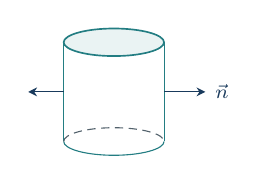
\begin{tikzpicture}[handout diagram,x=0.75cm,y=0.7cm]
\draw[accent] (-0.85,0) -- (-0.85,1.8) (0.85,0) -- (0.85,1.8);
 \path[region] (0,1.8) ellipse (0.85 and 0.25);
 \draw[accent] (-0.85,0) arc[start angle=180,end angle=360,x radius=0.85,y radius=0.25];
 \draw[guide] (-0.85,0) arc[start angle=180,end angle=0,x radius=0.85,y radius=0.25];
 \draw[->,ink] (0.85,0.9) -- (1.55,0.9) node[right] {$\vec n$};
 \draw[->,ink] (-0.85,0.9) -- (-1.45,0.9);
\end{tikzpicture}\par
{\small\color{muted}円柱側面は軸から外へ}\par
\end{minipage}\hfill
\begin{minipage}[b]{0.31\linewidth}\centering
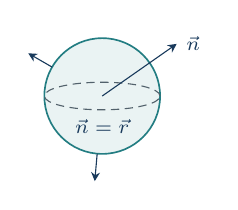
\begin{tikzpicture}[handout diagram,x=0.7cm,y=0.7cm]
\path[region] (0,0) circle (1.05);
 \draw[guide] (0,0) ellipse (1.05 and 0.25);
 \draw[->,ink] (0,0) -- (35:1.65) node[right] {$\vec n$};
 \draw[->,ink] (150:1.05) -- (150:1.55);
 \draw[->,ink] (265:1.05) -- (265:1.55);
 \node at (0,-0.55) {$\vec n=\vec r$};
\end{tikzpicture}\par
{\small\color{muted}単位球面では半径方向が外向き}\par
\end{minipage}\hfill
\begin{minipage}[b]{0.31\linewidth}\centering
\begin{tikzpicture}[handout diagram,x=0.8cm,y=0.7cm]
\path[region] (0,0) ellipse (1.2 and 0.4);
 \draw[accent,->,semithick] (1.2,0) arc[start angle=0,end angle=155,x radius=1.2,y radius=0.4];
 \draw[->,ink,semithick] (0,0) -- (0,1.5) node[above] {$+z$};
 \node[below] at (0,-0.75) {$+z$ 側から見る};
\end{tikzpicture}\par
{\small\color{muted}上向き法線なら境界は反時計回り}\par
\end{minipage}
\par\vspace{2pt}

\end{minipage}\par\nointerlineskip
% Keep the exercises and writing space in the lower half of page 2.
\noindent\begin{minipage}[b][0.5\textheight][t]{\linewidth}
\exercises
\begin{problems}
\item $(-1,1)$ から $(0,1)$ への線分と、その逆向きの線分をそれぞれ媒介変数で表せ。$0\le t\le1$ を用いること。
\problemspace

\item $a,b>0$ の楕円 $x^2/a^2+y^2/b^2=1$ を、反時計回り・時計回りの両方で表せ。$t=0$ での位置と速度で向きを確認せよ。
\problemspace

\item $z=x^2+y^2$、$x^2+y^2\le1$ の曲面を上向きに表し、接ベクトル・単位法線・面積要素を求めよ。
\problemspace

\item 半径 $R>0$、高さ $H>0$ の円柱側面を外向きに表し、外積を計算せよ。パラメータの順序を交換すると何が変わるか。
\problemspace

\item 単位球面の表示 $\vec r(\alpha,\theta)=(\sin\alpha\cos\theta,\sin\alpha\sin\theta,\cos\alpha)$ の外積を計算し、外向きであることを確かめよ。極をどう扱うかも説明せよ。
\problemspace

\item 単位立方体の上面 $z=1$ と下面 $z=0$ を外向きに向き付ける。それぞれの境界を $+z$ 側から見ると、正の向きは時計回りか反時計回りか。理由も述べよ。
\problemspace
\end{problems}
\end{minipage}

\newpage
\handouttitle{第12回\quad 演習問題の解答}
{\small 設定した範囲と条件も確認しながら、計算を振り返ろう。}\par
\begin{problems}
\setlength{\itemsep}{7pt}
\item 順向きは $\vec r(t)=(-1+t,1)$、逆向きは $\widetilde{\vec r}(t)=(-t,1)$
（どちらも $0\le t\le1$）。速度はそれぞれ $(1,0)$、$(-1,0)$ である。

\item $0\le t\le2\pi$ として
$$
 \vec r_+(t)=(a\cos t,b\sin t),\qquad
 \vec r_-(t)=(a\cos t,-b\sin t).
$$
どちらも $t=0$ の位置は $(a,0)$。速度は $(0,b)$ と $(0,-b)$ なので、
右端から上へ進む前者が反時計回り、下へ進む後者が時計回りとなる。

\item $\vec r(x,y)=(x,y,x^2+y^2)$（$x^2+y^2\le1$）とおくと
$$
 \vec r_x=(1,0,2x),\quad \vec r_y=(0,1,2y),\quad
 \vec N=(-2x,-2y,1).
$$
第3成分が正なので上向きであり、
$$
 \vec n=\frac{(-2x,-2y,1)}{\sqrt{1+4x^2+4y^2}},\qquad
 dS=\sqrt{1+4x^2+4y^2}\,dx\,dy.
$$

\item $\vec r(\theta,z)=(R\cos\theta,R\sin\theta,z)$、
$0\le\theta<2\pi$、$0\le z\le H$ とすれば
$$
 \vec r_\theta=(-R\sin\theta,R\cos\theta,0),\quad \vec r_z=(0,0,1),\quad
 \vec r_\theta\times\vec r_z=(R\cos\theta,R\sin\theta,0).
$$
軸から外へ向くので外向き。順序を交換すると内向きとなるが、$dS=R\,d\theta\,dz$ の大きさは同じ。

\item 接ベクトルと外積は
$$
 \begin{aligned}
 \vec r_\alpha&=(\cos\alpha\cos\theta,\cos\alpha\sin\theta,-\sin\alpha),\\
 \vec r_\theta&=(-\sin\alpha\sin\theta,\sin\alpha\cos\theta,0),\\
 \vec r_\alpha\times\vec r_\theta&=\sin\alpha\,\vec r.
 \end{aligned}
$$
$0<\alpha<\pi$ では $\sin\alpha>0$ なので外向きで、$dS=\sin\alpha\,d\alpha\,d\theta$。
極は表示が退化するだけなので、別の局所表示で覆える。面積分では面積0の2点を除いて計算してよい。

\item 上面の外向き法線は $+z$ 方向なので、境界は $+z$ 側から見て反時計回り。
下面の外向き法線は $-z$ 方向なので、同じ $+z$ 側から見ると時計回りである。
法線を親指に合わせた右手の指の曲がる方向が、各境界の正の向きとなる。
\end{problems}
\keybox{法線を指定された向きに合わせてから境界を決めよう。外積を交換したとき、法線と流束の符号は反転し、面積は変わらない。}
\end{document}
